\documentclass[10pt,letterpaper]{article}

\usepackage{outlines}
\usepackage{amsmath}
\usepackage{tikz}
\usepackage{hyperref}
\usepackage{enumitem}
\usepackage{caption}
\usepackage{subcaption}
\DeclareCaptionOptionNoValue{centering}{\centering} % Make sure everything is centered in subs
\captionsetup[sub]{centering}

\usepackage{multirow}
\usepackage{cancel}
\usepackage{float}

\usepackage{parskip}

\usepackage{slantsc,lmodern}

\usepackage{pgfplotstable,booktabs}
\usepackage{textcomp}
\usepackage{gensymb}

\usepackage{paralist}

\usepackage{amsmath}
\usepackage{tikz}
\usepackage{hyperref}

\usepackage{pst-node}
\usepackage{auto-pst-pdf}

\usepackage[paper=a4paper,margin=1in]{geometry}

\makeatletter
\g@addto@macro\@floatboxreset\centering
\makeatother

\newcommand{\volume}{{\ooalign{\hfil$V$\hfil\cr\kern0.08em--\hfil\cr}}}




\author{Thaddeus Hughes \\ hughes.thad@gmail.com \\ thaddeus-maximus.github.io}
\date{\today}
\title{Generalized Beam Deflection Calculator}

\begin{document}
	\maketitle
	
	\begin{abstract}
		Beams are common structures for structural analysis. As such many analytical formulas for specific use cases exist. Complex cases can also be computed by use of static superposition, or the utilization of a finite-element (FE) model. I created a web interface for a rudimentary beam FE model.
	\end{abstract}

	\section{How does FE work?}

	A finite-element model works generally by solving a matrix equation of the form

	\begin{align}
		\{F\} = [K]\{q\} .
	\end{align}

	Where ${F}$ is the \textit{load vector}, $[K]$ is the \textit{stiffness matrix}, and ${q}$ is the \textit{displacement vector}. This may be recognized as simply a matrix form of a spring equation- which it is! The FE model works by splitting a large component into several small springs (\textit{elements}) with endpoints (\textit{nodes}).

	There are a few methods to solve this equation. One simple one is to multiply both sides by the matrix inverse (since there is no direct equivalent of division with matrices). This method does not scale well- but it works with the few elements we will need for this calculator.

	\begin{align}
		[K]^{-1} \{F\} = [K]^{-1} [K]\{q\} = \{q\}
	\end{align}

	There are many different forms of stiffness, depending on the exact element used.

	\section{Elements}

	We will use a 2D beam element derived from \textit{Euler-Bernoulli beam theory}. This element has four degrees of freedom: vertical deflection $v$ and rotation $\psi$ at each end node.

	\begin{figure}[H]
	\begin{tikzpicture}[x=0.8in,y=0.8in]
		\draw[darkgray, ultra thick] (-2,-.5) -- (-2,.5) -- (2,.5) -- (2,-.5) -- cycle;
		\draw[black, ultra thick, ->] (-2.6,-0.6) -- (-2.6,0.6) node[pos=0.5, left]{$v_1$};
		\draw[black, ultra thick, ->] (+2.6,-0.6) -- (+2.6,0.6) node[pos=0.5, right]{$v_2$};
		\draw[black, ultra thick, ->] (-1.7,0) arc(0:230:0.3) node[pos=0.2, right]{$\psi_1$};
		\draw[black, ultra thick, ->] (2.3,0) arc(0:230:0.3) node[pos=0.2, right]{$\psi_2$};
		\fill[black] (2,0) circle (0.05);
		\fill[black] (-2,0) circle (0.05);
	\end{tikzpicture}
	\caption{A beam with a fixed support, a pinned support, and a force load.}
	\end{figure}

	It can be found that the equation derived from euler-bernoulli beam theory is

	\begin{align}
		\begin{Bmatrix}
			F_1 \\
			M_1 \\
			F_2 \\
			M_2 
		\end{Bmatrix} = 
		\begin{bmatrix}
			12  & 6L   & -12 & 6L   \\
			6L  & 4L^2 & -6L & 2L^2 \\
			-12 & -6L  & 12  & -6L  \\
			6L  & 2L^2 & -6L & 4L^2 
		\end{bmatrix}
		\begin{Bmatrix}
			v_1 \\
			\psi_1 \\
			v_2 \\
			\psi_2 
		\end{Bmatrix}
	\end{align}

	This is just one element though! How do we link the elements together?

	\section{Direct Assembly}

	One simple way is by \textit{direct assembly}. It can be noticed that (roughly) the matrix looks something like

	\begin{align}
		\begin{Bmatrix}
			F_1 \\
			F_2 
		\end{Bmatrix} = 
		\begin{bmatrix}
			K & -K \\
			-K & K 
		\end{bmatrix}
		\begin{Bmatrix}
			u_1 \\
			u_2 
		\end{Bmatrix}
	\end{align}

	If we had two elements linked together like so:

	\begin{figure}[H]
	\begin{tikzpicture}[x=0.4in,y=0.4in]
		\draw[darkgray, ultra thick] (-2,-.5) -- (-2,.5) -- (2,.5) -- (2,-.5) -- cycle;
		\draw[darkgray, ultra thick] (2,-.5) -- (2,.5) -- (6,.5) -- (6,-.5) -- cycle;
		\node[black] at (0,0) {A} ;
		\node[black] at (4,0) {B} ;
		\fill[black] (-2,0) circle (0.1) node[left]{1};
		\fill[black] (2,0)  circle (0.1) node[left]{2};
		\fill[black] (6,0)  circle (0.1) node[left]{3};
	\end{tikzpicture}
	\caption{Two connected beams.}
	\end{figure}

	These two beams share node 2. That is to say, they both see the forces from node 2, and the deflection at node 2. This leads us to combine the equations for each element as so:

	\begin{align}
		\begin{Bmatrix}
			F_1 \\
			F_2 \\
			F_3 
		\end{Bmatrix} = 
		\begin{bmatrix}
			K_A  & -K_A    & 0    \\
			-K_A & K_A+K_B & -K_B \\
			0    & -K_B    & K_B
		\end{bmatrix}
		\begin{Bmatrix}
			u_1 \\
			u_2 \\
			u_3 
		\end{Bmatrix}
	\end{align}

	We're getting close to a problem we can solve! We've linked the nodes together, but we now need to constrain them. These beams are currently floating in space- we need to anchor them otherwise our displacements are meaningless (and, the matrix $[K]$ is singular and unsolvable). For example, let's apply the constraint that node 1 is fixed; that is, $u_1$ = 0. As a result, the associated column in $[K]$ (the first column) does not matter. Any loads applied to the node also do not matter since they would be absorbed by the fixed constraint. This allows us to remove columns and rows 1 of the stiffness matrix, degrees of freedom 1, and load 1, changing our equation to:

	\[
	\begin{pspicture} 
		\begin{Bmatrix}
			\rnode{A}{F_1} \\
			F_2 \\
			F_3 
		\end{Bmatrix} = 
		\begin{bmatrix}
			\rnode{C}{K_A}  & -K_A    & 0    \\
			-K_A & K_A+K_B & -K_B \\
			\rnode{D}{0}    & -K_B    & K_B
		\end{bmatrix}
		\begin{Bmatrix}
			\rnode{B}{u_1} \\
			u_2 \\
			u_3 
		\end{Bmatrix}
		\ncline{A}{B}
		\ncline{C}{D}
	\end{pspicture}
	\]

	\begin{align}
		\begin{Bmatrix}
			F_2 \\
			F_3 
		\end{Bmatrix} = 
		\begin{bmatrix}
			K_A+K_B & -K_B \\
			-K_B    & K_B
		\end{bmatrix}
		\begin{Bmatrix}
			u_2 \\
			u_3 
		\end{Bmatrix}
	\end{align}

	At this point we could plug in values $F_2$ and $F_3$, and solve with the matrix inverse method.

	\section{Applying to Beams}

	Let's show how this would work with a beam. Consider the following example:
	
	\begin{figure}[H]
	\begin{tikzpicture}[x=1.0in,y=1.0in]
		\draw[gray] (0, 0.05) -- (0, 0.3) node[pos=1, above]{$0$};
		\draw[gray] (1, 0.05) -- (1, 0.3) node[pos=1, above]{$L$};
		\draw[gray] (2, 0.05) -- (2, 0.3) node[pos=1, above]{$2L$};
		\draw[gray] (3, 0.05) -- (3, 0.3) node[pos=1, above]{$3L$};
		\draw[gray] (4, 0.05) -- (4, 0.3) node[pos=1, above]{$4L$};
		\draw[darkgray, ultra thick] (0,0) -- (4,0);
		\draw[blue, ultra thick, ->] (3,-0.05) -- (3,-0.3) node[pos=0.5, right]{W};
		\fill[black, ultra thick] (0.9,0) -- (1.1,0) -- (1.1,-0.2) -- (0.9,-0.2) -- cycle;
		\fill[black, ultra thick] (2,0) -- (2.1,-0.2) -- (1.9,-0.2) -- cycle;
	\end{tikzpicture}
	\caption{A beam with a fixed support, a pinned support, and a force load.}
	\end{figure}

	We can start by creating a general stiffness matrix with the general assembly method:

	\begin{align}
		[K] = 
		\begin{bmatrix}
12 & 6L & -12 & 6L & & & & & & \\
6L & 4L^2 & -6L & 2L^2 & & & & & & \\
-12 & -6L & 24 & 12L & -12 & 6L & & & & \\
6L & 2L^2 & 12L & 8L^2 & -6L & 2L^2 & & & & \\
 & & -12 & -6L & 24 & 12L & -12 & 6L & & \\
 & & 6L & 2L^2 & 12L & 8L^2 & -6L & 2L^2 & & \\
 & & & & -12 & -6L & 24 & 12L & -12 & 6L \\
 & & & & 6L & 2L^2 & 12L & 8L^2 & -6L & 2L^2 \\
 & & & & & & -12 & -6L & 12 & -6L \\
 & & & & & & 6L & 2L^2 & -6L & 4L^2
		\end{bmatrix}
	\end{align}

	(Zeroes have been omitted from matrix to aid in readability)

	The load vector is:

	\begin{align}
		{F} = 
		\begin{Bmatrix}
			F_1 \\
			M_1 \\
			F_2 \\
			M_2 \\
			F_3 \\
			M_3 \\
			F_4 \\
			M_4 \\
			F_5 \\
			M_5
		\end{Bmatrix} = 
		\begin{Bmatrix}
			0 \\
			0 \\
			0 \\
			0 \\
			-W \\
			0 \\
			0 \\
			0 \\
			0 \\
			0
		\end{Bmatrix}
	\end{align}

	Combining this yields:

	\begin{align} 
		\begin{Bmatrix}
			0 \\
			0 \\
			0 \\
			0 \\
			-W \\
			0 \\
			0 \\
			0 \\
			0 \\
			0
		\end{Bmatrix} = \begin{bmatrix}
12 & 6L & -12 & 6L & & & & & & \\
6L & 4L^2 & -6L & 2L^2 & & & & & & \\
-12 & -6L & 24 & 0 & -12 & 6L & & & & \\
6L & 2L^2 & 0 & 8L^2 & -6L & 2L^2 & & & & \\
 & & -12 & -6L & 24 & 0 & -12 & 6L & & \\
 & & 6L & 2L^2 & 0 & 8L^2 & -6L & 2L^2 & & \\
 & & & & -12 & -6L & 24 & 0 & -12 & 6L \\
 & & & & 6L & 2L^2 & 0 & 8L^2 & -6L & 2L^2 \\
 & & & & & & -12 & -6L & 12 & -6L \\
 & & & & & & 6L & 2L^2 & -6L & 4L^2
		\end{bmatrix} \begin{Bmatrix}
			v_1 \\
			\psi_1 \\
			v_2 \\
			\psi_2 \\
			v_3 \\
			\psi_3 \\
			v_4 \\
			\psi_4 \\
			v_5 \\
			\psi_5
		\end{Bmatrix}
	\end{align}

	The fixed support at node 2 removes degrees of freedom $v_2$, $\psi_2$. The pinned support at node 3 removes only $v_3$ (pin still permits rotation).

	\[
	\begin{pspicture} 
		\begin{Bmatrix}
			0 \\
			0 \\
			\rnode{A}{0} \\
			\rnode{C}{0} \\
			\rnode{E}{0} \\
			0 \\
			-W \\
			0 \\
			0 \\
			0
		\end{Bmatrix} = \begin{bmatrix}
12 & 6L & \rnode{G}{-12} & \rnode{I}{6L} & \rnode{K}{} & & & & & \\
6L & 4L^2 & -6L & 2L^2 & & & & & & \\
-12 & -6L & 24 & 0 & -12 & 6L & & & & \\
6L & 2L^2 & 0 & 8L^2 & -6L & 2L^2 & & & & \\
 & & -12 & -6L & 24 & 0 & -12 & 6L & & \\
 & & 6L & 2L^2 & 0 & 8L^2 & -6L & 2L^2 & & \\
 & & & & -12 & -6L & 24 & 0 & -12 & 6L \\
 & & & & 6L & 2L^2 & 0 & 8L^2 & -6L & 2L^2 \\
 & & & & & & -12 & -6L & 12 & -6L \\
 & & \rnode{H}{} & \rnode{J}{} & \rnode{L}{} & & 6L & 2L^2 & -6L & 4L^2
		\end{bmatrix} \begin{Bmatrix}
			v_1 \\
			\psi_1 \\
			\rnode{B}{v_2} \\
			\rnode{D}{\psi_2} \\
			\rnode{F}{v_3} \\
			\psi_3 \\
			v_4 \\
			\psi_4 \\
			v_5 \\
			\psi_5
		\end{Bmatrix}
		\psset{nodesep=-1.5ex, linewidth=0.4pt}
		\ncline{A}{B}
		\ncline{C}{D}
		\ncline{E}{F}
		\ncline{G}{H}
		\ncline{I}{J}
		\ncline{K}{L}
	\end{pspicture}
	\]

	\begin{align}
		\begin{Bmatrix}
			0 \\
			0 \\
			0 \\
			-W \\
			0 \\
			0 \\
			0
		\end{Bmatrix} = \begin{bmatrix}
12 & 6L & & & & & \\
6L & 4L^2 & & & & & \\
 & & 8L^2 & -6L & 2L^2 & & \\
 & & -6L & 24 & 0 & -12 & 6L \\
 & & 2L^2 & 0 & 8L^2 & -6L & 2L^2 \\
 & & & -12 & -6L & 12 & -6L \\
 & & & 6L & 2L^2 & -6L & 4L^2 
 		\end{bmatrix} \begin{Bmatrix}
			v_1 \\
			\psi_1 \\
			\psi_3 \\
			v_4 \\
			\psi_4 \\
			v_5 \\
			\psi_5
		\end{Bmatrix}
	\end{align}

	At this point, the matrix equation could be solved to achieve the nodal displacement vector.

	This tells us about the nodes, but what about inbetween areas?

	\section{Post Processing: Shape Functions}

	To derive the beam stiffness matrix, particular \textit{shape functions} were used (the Hermite shape functions). These are nondimensional equations that represent the contribution of one degree of freedom to the displacement field in an element. By combining these displacement fields, we can determine the total displacement field.

	\begin{figure}[H]
		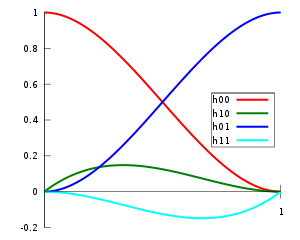
\includegraphics[width=0.5\textwidth]{hermite.png}
		\caption{Hermite shape functions}
	\end{figure}

	These hermite shape functions can be represented as:

	\begin{align}
		N = \begin{Bmatrix}
				\frac{1}{4} (1-\zeta^2 (2+\zeta) \\
				\frac{L}{8} (1-\zeta)^2 (\zeta+1) \\
				\frac{1}{4} (1+\zeta)^2 (2-\zeta) \\
				\frac{L}{8} (1+\zeta)^2 (\zeta-1) 
		\end{Bmatrix}^T
	\end{align}

	Where $L$ is the element length and $\zeta$ is a nondimensional parameter that is -1 at the left of the element, +1 at the right, and 0 in the center.

	\begin{align}
		\zeta = 2 \frac{x}{L} - 1
	\end{align}

	Where $x$ is the distance from the left of the element.

	The functions can be used to find the displacement field $v$:

	\begin{align}
		v = \{N\} \{q\} =
		\begin{Bmatrix}
				\frac{1}{4} (1-\zeta^2 (2+\zeta) \\
				\frac{L}{8} (1-\zeta)^2 (\zeta+1) \\
				\frac{1}{4} (1+\zeta)^2 (2-\zeta) \\
				\frac{L}{8} (1+\zeta)^2 (\zeta-1) 
		\end{Bmatrix}^T 
		\begin{Bmatrix}
			v_1 \\
			\psi_1 \\
			v_2 \\
			\psi_2 
		\end{Bmatrix}
	\end{align}

	This helps us plot the displacement field, but what about the slope, bending moment, and shear force?

	The slope $\theta$ is simply the derivative of the displacement field $v$ with respect to position $x$. The bending moment $M$ and shear force $V$ can also be found from Euler-Bernoulli beam theory.

	\begin{align}
		\theta &= \frac{d v}{d x} \\
		M      &= E I \frac{d^2 v}{d x^2} \\
		V      &= \frac{d}{d x} (E I \frac{d^2 v}{d x^2}) = E I \frac{d^3 v}{d x^3}
	\end{align}

	Assuming elastic modulus $E$ and second moment of area $I$ are constant over the element.

	To find these derivatives of $v$, we can use the shape functions, ignoring the nodal displacements since they do not vary with $x$.

	\begin{align}
		\frac{dv}{dx} = \frac{d}{dx} [\{N\} \{q\}] = \frac{d \{N\}}{dx} \{q\}
	\end{align}

	The chain rule can be used to help find these derivatives.

	\begin{align}
		\frac{d \{N\}}{d x} &= \frac{d \{N\}}{d \zeta} \frac{d \zeta}{d x} \\
		\frac{d^2 \{N\}}{d x^2} &= \frac{d^2 \{N\}}{d \zeta^2} (\frac{d \zeta}{d x})^2 + \frac{d \{N\}}{d \zeta} \frac{d^2 \zeta}{d x^2} \\
		\frac{d^3 \{N\}}{d x^3} &= \frac{d^3 \{N\}}{d \zeta^3} (\frac{d \zeta}{d x})^3 + 3 \frac{d^2 \{N\}}{d \zeta^2} \frac{d \zeta}{d x}\frac{d^2 \zeta}{d x^2} + \frac{d \{N\}}{d \zeta}\frac{d^3 \zeta}{d x^3}
	\end{align}

	Looks ugly! But luckily, the higher order derivatives of $\zeta$ are zero.

	\begin{align}
		\frac{d \zeta}{d x} &= \frac{2}{L} \\
		\frac{d^2 \zeta}{d x^2} = \frac{d^3 \zeta}{d x^3} &= 0
	\end{align}

	\begin{align}
		\frac{d \{N\}}{d x} &= \frac{d \{N\}}{d \zeta} \frac{2}{L} \\
		\frac{d^2 \{N\}}{d x^2} &= \frac{d^2 \{N\}}{d \zeta^2} (\frac{2}{L})^2 \\
		\frac{d^3 \{N\}}{d x^3} &= \frac{d^3 \{N\}}{d \zeta^3} (\frac{2}{L})^3
	\end{align}

	The shape function derivatives are

	\begin{align}
		\frac{d \{N\}}{d x}     =
		\begin{Bmatrix}
				\frac{3}{4} (\zeta^2-1) \frac{2}{L} \\
				\frac{L}{8} (3 \zeta^2-2 \zeta - 1) \frac{2}{L} \\
			   -\frac{3}{4} (\zeta^2-1) \frac{2}{L} \\
				\frac{L}{8} (3 \zeta^2+2 \zeta -1) \frac{2}{L}
		\end{Bmatrix}^T &
		\frac{d^2 \{N\}}{d x^2} =
		\begin{Bmatrix}
				\frac{6 \zeta}{L^2} \\
				\frac{3 \zeta-1}{L} \\
			   -\frac{6 \zeta}{L^2} \\
				\frac{3 \zeta+1}{L}
		\end{Bmatrix}^T &
		\frac{d^3 \{N\}}{d x^3} =
		\begin{Bmatrix}
				\frac{12}{L^3} \\
				\frac{6}{L^2} \\
			   -\frac{12}{L^3} \\
				\frac{6}{L^2}
		\end{Bmatrix}^T 
	\end{align}

	\section{Validation Examples}

	Comparison to analytical solutions is a necessary component when validating any FE model. \href{https://mechanicalc.com/reference/beam-deflection-tables}{\underline{MechaniCalc}} has some good analytical solutions I will compare to.

	\subsection{Cantilevered, Intermediate Load}

	\begin{figure}[H]
		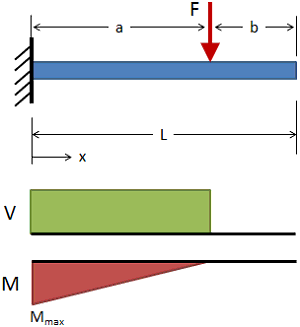
\includegraphics[width=0.5\textwidth]{beam_case1_schematic.png}
	\end{figure}

	Let $E = 69 GPa$, $L = 100 mm$, round bar with $d = 5 mm$, $F = 200 N$, $a = 60mm$.

	\begin{align}
		I = \frac{\pi}{64} d^4 = \frac{\pi}{64} (0.100 m)^4 = 3.06796 \times 10^{-11} m^4
	\end{align}
	\begin{align}
		\delta_{a} &= - \frac{F a^2}{6 E I} (3 L - a) &= - \frac{200 N \times (0.06 m)^2}{6 \times 69 GPa \times 30.6796 mm^4} (3 \times 0.06 m - 0.06 m) &= 6.802 mm\\
		\delta_{end} &= - \frac{F a^2}{6 E I} (3 L - a) &= - \frac{200 N \times (0.06 m)^2}{6 \times 69 GPa \times 30.6796 mm^4} (3 \times 0.1 m - 0.06 m) &= 13.6048 mm\\
		\theta_{a/2} &= - \frac{F (a/2)^2}{2 E I} (2 L - a/2) &= \frac{200 N \times .03 m}{2 \times 69 GPa \times 30.6796 mm^4} (2 \times 0.1m - .03m) = 7.305 \ deg\\
		& V_{0 \mbox{ to } a} &= F &= 200 \ N \\
		& M_{x=0} &= -F \times a = - 200 N \times .06 m &= - 12\ Nm
	\end{align}

	You can plug in the values to the calculator and verify this load case for yourself. I found all of the above numbers to be accurate.

	\subsection{Simply Supported, Center Moment}

	\begin{figure}[H]
		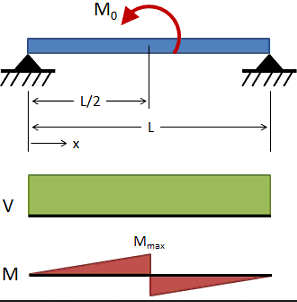
\includegraphics[width=0.5\textwidth]{beam_case2_schematic.png}
	\end{figure}

	Let $E = 27557 ksi$, $L = 6 in$, box bar with $w = 0.5 in$, $h = 2in$, $M = 1200 ft-lbf$.

	\begin{align}
		I = \frac{1}{12} b h^3 = 1/3 in^4
	\end{align}
	\begin{align}
		\delta_{x = 1.25 in} &= \frac{ - M x}{24 L E I}(L^2 - 4*x^2) &= \frac{-12\ ft\ lbf\ 1.25 \ in}{24 \times \ 6 \ in \ 27557 \ ksi \ 1/3 \ in^4} ((6 in)^2 - 4 (1.25 in)^2) &= -.4048 thou \\
		\theta_{1} &= \frac{- M L}{24 E I} &= \frac{-1200\ ft\ lbf\ 6 \ in}{24 \times \ 27557 \ ksi \ 1/3 \ in^4} &= -.02246 \ deg \\
		V &= M / L &= 1200 ft-lbf / 6 in &= 2400 lbf \\
		M_{x=L/2} &= M / 2 &= 1200 ft-lbf / 2 &= 600 ft-lbf
	\end{align}

	You can plug in the values to the calculator and verify this load case for yourself. I found all of the above numbers to be accurate.

\end{document}